\documentclass{sigchi}

% Use this section to set the ACM copyright statement (e.g. for
% preprints).  Consult the conference website for the camera-ready
% copyright statement.

% Copyright
\CopyrightYear{2021}
%\setcopyright{acmcopyright}
\setcopyright{acmlicensed}
%\setcopyright{rightsretained}
%\setcopyright{usgov}
%\setcopyright{usgovmixed}
%\setcopyright{cagov}
%\setcopyright{cagovmixed}
% DOI
\doi{https://doi.org/10.1145/3313831.XXXXXXX}
% ISBN
\isbn{XXX-X-XXXX-XXXX-X/21/05}
%Conference
\conferenceinfo{CHI'21,}{May 8--13, 2021, Yokohama, Japan}
%Price
%\acmPrice{\$15.00}

% Use this command to override the default ACM copyright statement
% (e.g. for preprints).  Consult the conference website for the
% camera-ready copyright statement.

%% HOW TO OVERRIDE THE DEFAULT COPYRIGHT STRIP --
%% Please note you need to make sure the copy for your specific
%% license is used here!
% \toappear{
% Permission to make digital or hard copies of all or part of this work
% for personal or classroom use is granted without fee provided that
% copies are not made or distributed for profit or commercial advantage
% and that copies bear this notice and the full citation on the first
% page. Copyrights for components of this work owned by others than ACM
% must be honored. Abstracting with credit is permitted. To copy
% otherwise, or republish, to post on servers or to redistribute to
% lists, requires prior specific permission and/or a fee. Request
% permissions from \href{mailto:Permissions@acm.org}{Permissions@acm.org}. \\
% \emph{CHI '16},  May 07--12, 2016, San Jose, CA, USA \\
% ACM xxx-x-xxxx-xxxx-x/xx/xx\ldots \$15.00 \\
% DOI: \url{http://dx.doi.org/xx.xxxx/xxxxxxx.xxxxxxx}
% }

% Arabic page numbers for submission.  Remove this line to eliminate
% page numbers for the camera ready copy
% \pagenumbering{arabic}

% Load basic packages
\usepackage{balance}       % to better equalize the last page
\usepackage{graphics}      % for EPS, load graphicx instead 
\usepackage[T1]{fontenc}   % for umlauts and other diaeresis
\usepackage{txfonts}
\usepackage{mathptmx}
\usepackage[pdflang={en-US},pdftex]{hyperref}
\usepackage{color}
\usepackage{booktabs}
\usepackage{textcomp}
\usepackage{lipsum}

% Some optional stuff you might like/need.
\usepackage{microtype}        % Improved Tracking and Kerning
% \usepackage[all]{hypcap}    % Fixes bug in hyperref caption linking
\usepackage{ccicons}          % Cite your images correctly!
% \usepackage[utf8]{inputenc} % for a UTF8 editor only

% If you want to use todo notes, marginpars etc. during creation of
% your draft document, you have to enable the "chi_draft" option for
% the document class. To do this, change the very first line to:
% "\documentclass[chi_draft]{sigchi}". You can then place todo notes
% by using the "\todo{...}"  command. Make sure to disable the draft
% option again before submitting your final document.
\usepackage{todonotes}

% Paper metadata (use plain text, for PDF inclusion and later
% re-using, if desired).  Use \emtpyauthor when submitting for review
% so you remain anonymous.
\def\plaintitle{Lifestyle and study equipment changes during distance learning}
\def\plainauthor{First Author, Second Author, Third Author,
  Fourth Author, Fifth Author, Sixth Author}
\def\emptyauthor{}
\def\plainkeywords{distance learning; student; home office; study environment; work environment; motivation; pandemic; health; }
\def\plaingeneralterms{Documentation, Standardization}

% llt: Define a global style for URLs, rather that the default one
\makeatletter
\def\url@leostyle{%
  \@ifundefined{selectfont}{
    \def\UrlFont{\sf}
  }{
    \def\UrlFont{\small\bf\ttfamily}
  }}
\makeatother
\urlstyle{leo}

% To make various LaTeX processors do the right thing with page size.
\def\pprw{8.5in}
\def\pprh{11in}
\special{papersize=\pprw,\pprh}
\setlength{\paperwidth}{\pprw}
\setlength{\paperheight}{\pprh}
\setlength{\pdfpagewidth}{\pprw}
\setlength{\pdfpageheight}{\pprh}

% Make sure hyperref comes last of your loaded packages, to give it a
% fighting chance of not being over-written, since its job is to
% redefine many LaTeX commands.
\definecolor{linkColor}{RGB}{6,125,233}
\hypersetup{%
  pdftitle={\plaintitle},
% Use \plainauthor for final version.
%  pdfauthor={\plainauthor},
  pdfauthor={\emptyauthor},
  pdfkeywords={\plainkeywords},
  pdfdisplaydoctitle=true, % For Accessibility
  bookmarksnumbered,
  pdfstartview={FitH},
  colorlinks,
  citecolor=black,
  filecolor=black,
  linkcolor=black,
  urlcolor=linkColor,
  breaklinks=true,
  hypertexnames=false
}

% create a shortcut to typeset table headings
% \newcommand\tabhead[1]{\small\textbf{#1}}

% End of preamble. Here it comes the document.
\begin{document}
\title{\plaintitle}
\numberofauthors{4}
\author{
  \alignauthor{Author One\\
    \affaddr{for Submission}\\
    \affaddr{}\\
    \email{}}\\
  \alignauthor{Author Two\\
    \affaddr{for Submission}\\
    \affaddr{}\\
    \email{}}\\
  \alignauthor{Author Three\\
    \affaddr{for Submission}\\
    \affaddr{}\\
    \email{}}\\
  \alignauthor{Author Four\\
    \affaddr{for Submission}\\
    \affaddr{}\\
    \email{}}\\
}
\maketitle
\begin{abstract}
Given the appearance of the new pathological risk incurred during the 2020 Covid-19 pandemic, most educational institutions, be them either lower or higher educational, have had to restrict their activity on-campus and promote a fully online pedagogical methodology in order to avoid the spread of the virus and protect the health of both students and teachers. By employing already existing software solutions to the likes of \emph{Zoom}, \emph{Microsoft Teams}, and other existing tools, courses have been completely moved within the realm of the internet to the best of the ability of each educational institution. In this context, the authors are trying to investigate the effects that the sudden move to distance learning has had on students from different backgrounds, as well as how they have been forced to change their study and work environment to cope with the perpetual stress of academic life within the confines of their own home.
\end{abstract}


% ACM Classfication

\begin{CCSXML}
<ccs2012>
<concept>
<concept_id>10003456.10003457.10003527.10003542</concept_id>
<concept_desc>Social and professional topics~Adult education</concept_desc>
<concept_significance>500</concept_significance>
</concept>
<concept>
<concept_id>10003120.10003121</concept_id>
<concept_desc>Human-centered computing~Human computer interaction (HCI)</concept_desc>
<concept_significance>500</concept_significance>
</concept>
<concept>
<concept_id>10003120.10003121.10003122.10003334</concept_id>
<concept_desc>Human-centered computing~User studies</concept_desc>
<concept_significance>100</concept_significance>
</concept>
</ccs2012>
\end{CCSXML}

\ccsdesc[500]{Social and professional topics~Adult education}
\ccsdesc[300]{Human-centered computing~Human computer interaction (HCI)}
\ccsdesc[100]{Human-centered computing~User studies}

% Author Keywords
\keywords{\plainkeywords}

% Print the classification codes
\printccsdesc



\section{Introduction}

At the start of 2020, most countries around the world have had to impose strict restriction upon public spaces and institution in order to combat the eventual spread of Covid-19 within their populations. One measure imposed upon the educational systems was to forbid as much as possible lectures and other educational activities within their campuses as to avoid unnecessary and possible life-threatening contact between members of the institutions. In order to continue with the already started semester, most if not all education institutions have put forward online procedures based on already existing infrastructure in order for courses to still take place. Students have suddenly found themselves studying full time from the comfort of their home, not needing to travel to the universities campuses anymore. During their own experiences as students within the Summer 2020 semester, the authors have notice certain trends within their own behaviour and that of fellow students related to the unpreparedness of their own home-study environment and the rising motivational issues, and so, decided to perform an inquiry under the course work for the User Research Methods PR at the Technical University of Vienna, in order to investigate if indeed there was a general unpreparedness across the student population for such a drastic move to distance learning, as well as, if there is such a notion as a \emph{perfect study environment}, and in the end, conclude with a small \emph{tips and tricks} handbook which other students might find helpful in order to increase their comfort and motivation for studying at home and eventually decrease the amount of stress cause by social isolation.\cite{fauci_lane_redfield_2020, hossain_mental_2020}


\section{Related Work}

Here we should probably talk about the previous papers we read about distance learning, social isolation, education during other pandemics, as well as papers about the research methodologies.

\section{Methods}

\subsubsection{Research Questions}


\subsection{Methodologies}
In order to perform their research as best as possible, the authors have decided on utilizing three separate methodologies in order to achieve a coherent approach and take into account as many aspects related towards \emph{study environments} as possible. They started by performing auto-ethnography upon themselves to have an introspective look over their own experience during the first and second semesters of their studies within the context of the pandemic restrictions. Using the findings of the auto-ethnography, they have arrived at a number of interview questions that where used in a series of semi-structured interviews with participants outside of the research team. Ending by performing an photographic ethnography of pictures taken by the same interview participants in order to analyse them in parallel with the interview transcriptions and achieve a more coherent image of each participants actual study environments.

\subsubsection{Auto-ethnography}

Before starting the auto-ethnography research, each researcher has been given an information sheet and consent form which had to be sign by the research-participant and one of the other researchers. The structure of the document has been agreed upon unanimously by the team as so to avoid any potential issues related to data privacy of the resulting documents from the auto-ethnographic research.

After signing the consent form, each researcher has had to conduct an inner-inquiry upon his or hers experience that resulted from the drastic change towards full-time studying from home, as well as making a comparison between their study/work environment and study workload between their previous semester (e.g. Winter 2019/2020) and the next restricted semesters (e.g. Summer 2020, Winter 2020/2021).

Upon finishing their report about their own experience, each researcher had to take a picture of their current study environment/s (see Figure~\ref{fig:figure1} as an example) and attach it to the report. Afterwards all reports where analysed by each researcher, and researcher-participant had to perform a presentation of their experience to all other researchers. Findings culminating in organizing the information using thematic analysis using Miro\footnote{\url{https://miro.com/}} and extracting possible interview questions for their findings. After having decided on the possible interview questions, sample semi-structured interview took place, having one of the researchers as a participant, and two others as interviewer and observer. Upon finishing the sample interview, the interview question had been filtered to only five central questions as so to provide a structure for the incoming participant interviews.
\begin{figure}
\centering
  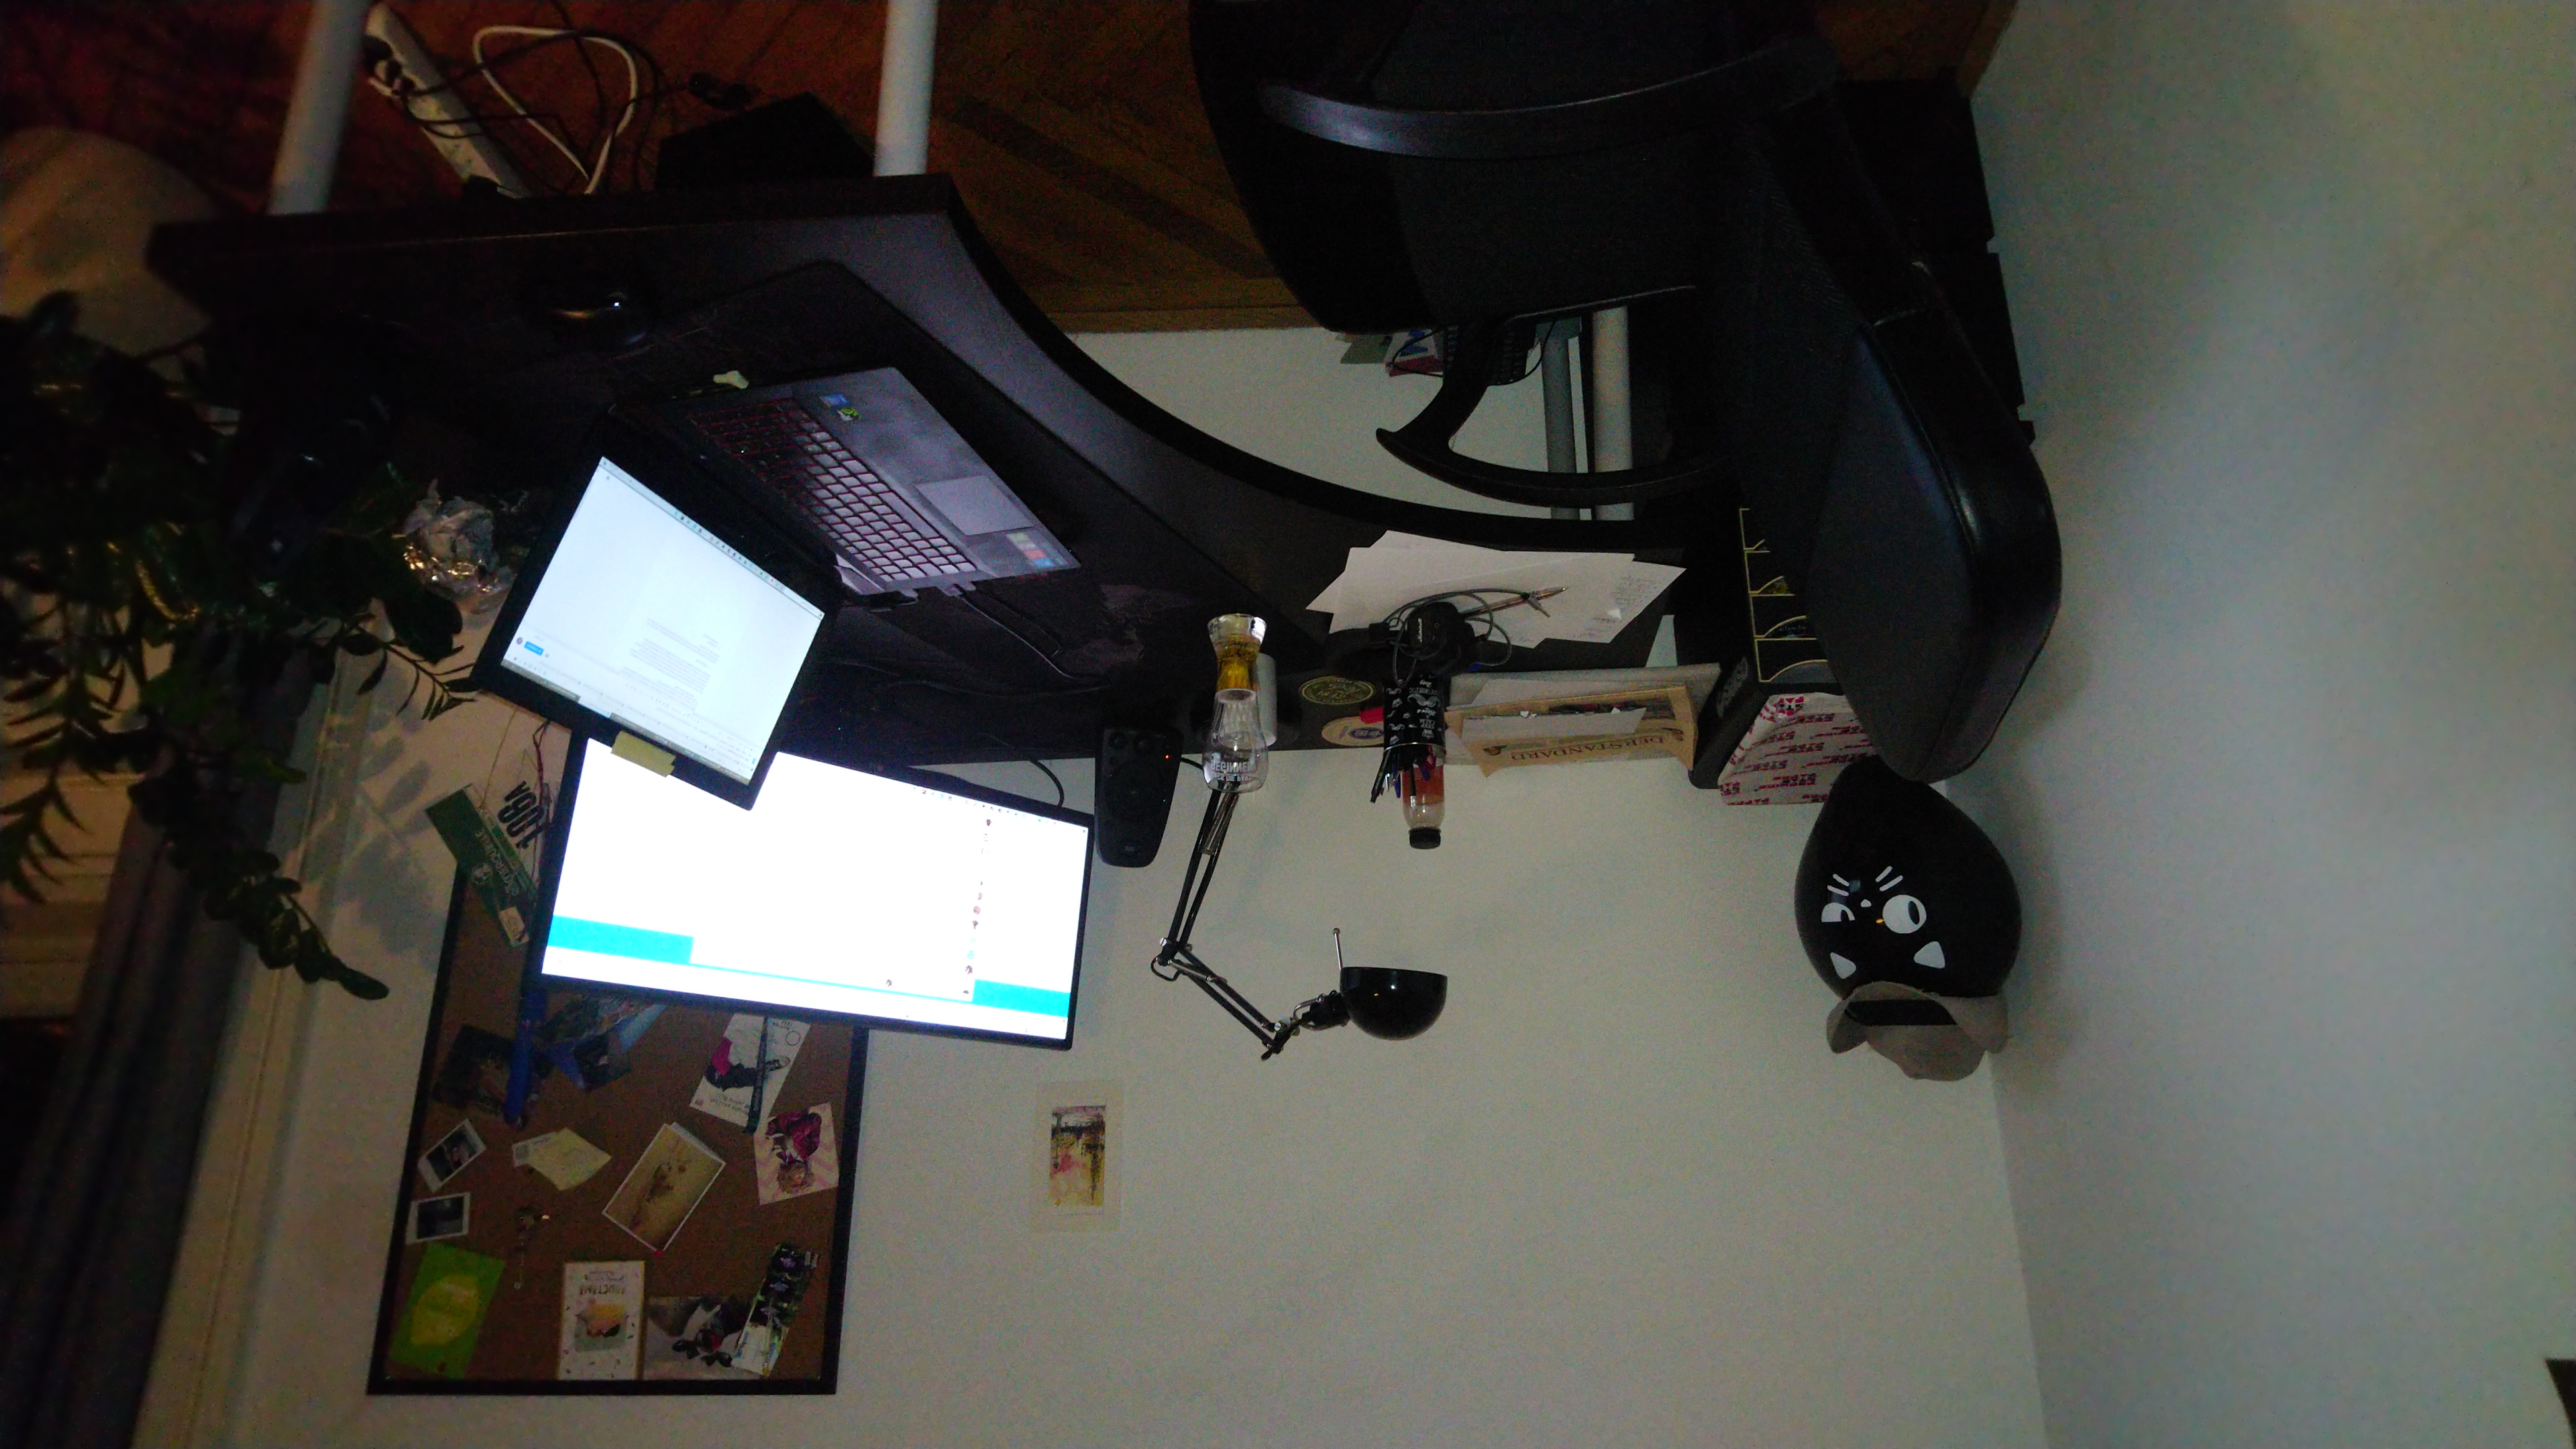
\includegraphics[width=0.9\columnwidth]{figures/auto-e-picture}
  \caption{Sample picture from the Auto-Ethnographic method, showing the desk of one of the researchers}~\label{fig:figure1}
\end{figure}

\subsubsection{Semi-structured Interviews}
The 5 interview questions
Who were the participants (general information), where the interviews were taken, how we found the participants, age, academic status, consent management, tools, analysing the interview, miro idea board / extracting data THEMATIC ANALYSING 

Some people did not know how the pandemic will evolve so they did not prepare for a long home learning situation, we asked them how the ideal setup will look like or if they know the next semesters  will be remotely what will they change.

issues: Single interviewer, no observer., subjectivity issues due to the participants being friends

\subsubsection{Photographic Ethnography}
Using the photo analysis method, the researches wanted to discover the study setups of students engaged in distance learning. The method was chose to give a better overview of essential items used by students for improving the health and comfort during online studies, at home. The participants agreed on sending a photo of their environment before the semi-structured online interviews. Moreover, the researchers shared photos of their personal setups used for remote studies. Two consents were used in the research: one sent to the participants before the semi-structured online interview, and another, for the researchers themselves, before starting the auto-ethnography process. The processes of storing, analyzing, anonymizing and deletion of the participants and researchers photos were covered in the mentioned consents.

As visual recording of the personal space …, not all the participants agreed to expose their working space. A number of X photos was collected in the photo analysis process. A visual difference between the state of the learning environment before and after switching to distance learning could not been made, as the photos received by the researchers were taken in the actual context of the pandemic. Only one participant sent photos of their old and their actual setup.  One participant sent a photo of their current setup, and two photos of setups that could serve as inspiration for their ideal setup. All photos received by the participants were used in the analyze process.

\begin{figure}
\centering
  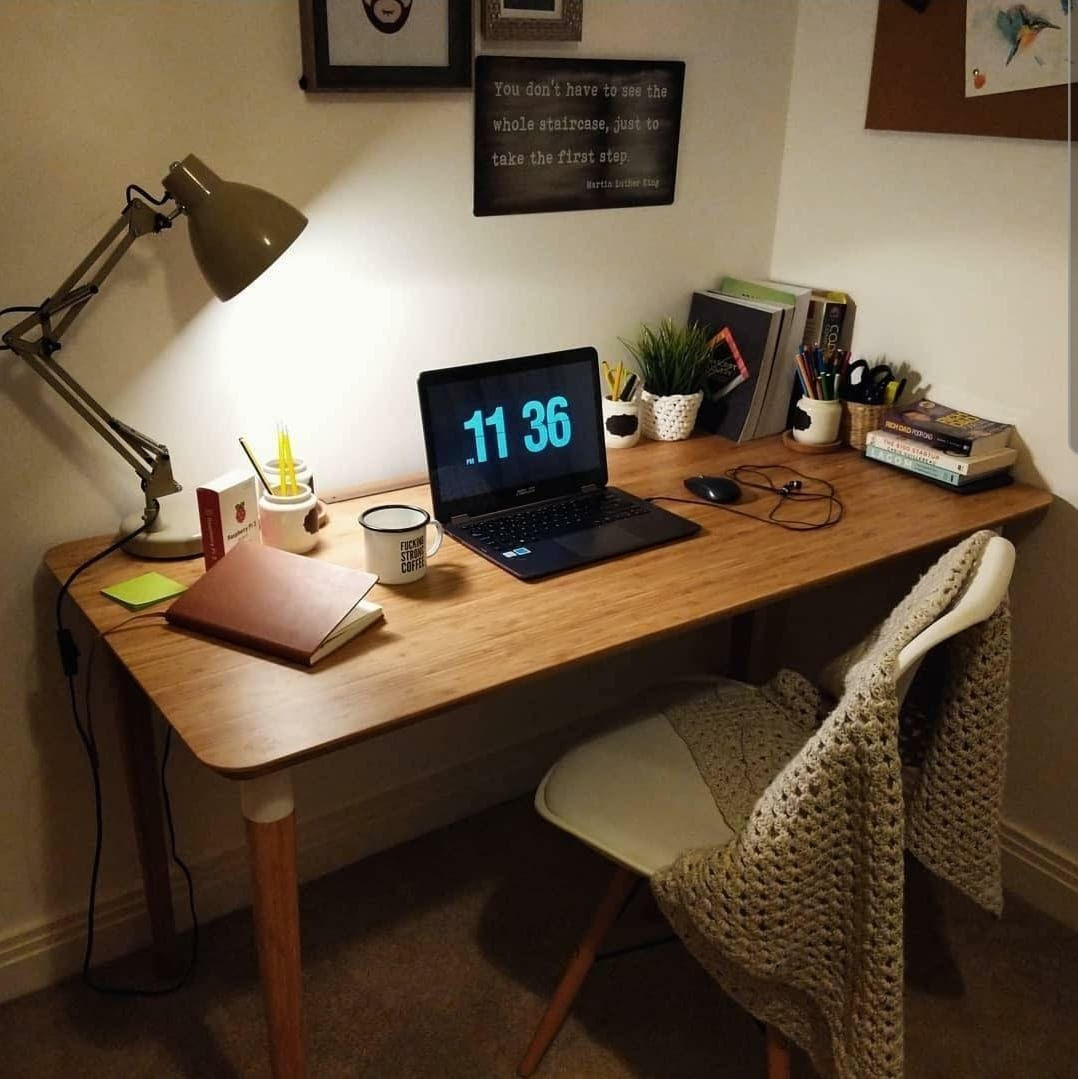
\includegraphics[width=0.9\columnwidth]{figures/perfect-setup}
  \caption{A sample photo from the Photographic Ethnography method given by one of the participants, it is the desired "perfect study environment''}~\label{fig:figure1}
\end{figure}

\section{Findings}

We need to talk about the research question results here.

Our findings from the interviews

Our findings from the photos: Both participants and from the auto-ethnography 


The analyze of the photos received from the participants and from the researchers involved in the study, showed unique, personalized study environments,  with a commune focus on ergonomics, efficiency and aesthetics. The result showed that the position of the working desk is usually located close to a direct source of natural light.  The importance of a natural source of light was mentioned by several participants during the semi-structured online interview process. Items such as: second screen, laptop, lamp, plants, notebooks were … 

\section{Discussion}

Things to talk about: 
1.Universities could open libraries or study spaces. Even increase the amount of space post-pandemic, as an issue already existed
2. Items that are we recommend to use for study and the uni should give discounts to
3. 

\subsection{Limitations}

\section{Implications for design}

It is worth noting that the research presented within this paper is not meant necessarily to provide the HCI community with a new form of interaction or a profoundly new methodological approach in how human-computer interaction can be studied, but it is meant to be seen more through the lens of \cite{dourish_implications_2006} where the significance of \emph{``Implications for design''} stems from observing human habits within a highly isolated scenario where most of the study and work interactions are perpetuated solely through technology. The authors desire is not to emphasize the need for bigger screens, or more comfortable chairs, but to show how much of our lives \emph{can} be replaced through software.

\subsection{Office of the next pandemic}

Given our interviews with the participants, no clear generalizing statement can be drawn on previous study setups possessed before the enactment of social distancing norms. But several have attributed a more aware understanding of the need to have such an environment within their homes. 
Noticing the likely-hood of our current situation to continue for at least one more semester, multiple participants had come to the conclusion and indeed already have plans of improving their study and work environments. Putting in question if a need in providing highly economical solutions in so as to reduce the overall cost of creating such a setup might be the next and most valuable step for the industry to take.

\subsection{Replacement of social interaction}

Multiple participants have expressed an inner desired to talk about their motivational issues while studying in this new environment. And to our amazement, different solutions in coping have been applied by each, from simple \emph{Zoom} study meetups, to arguably illegal (though depending on the country, might not be) face-to-face lecture viewings. Here the authors would like to express that a proper replacement of the in-class lecture experience, still does not exist and some participants have even emphasized a small regress due to the constant gap in interactivity that distance learning cannot overcome.

\section{Conclusions and future work}

1. A study on a more diverse group of students
2. A more in-depth study about motivational aspects
3. West country rich 
4. Didn’t realize the length of the pandemic
5. What could the regulations look like?
6. Maybe (?) we have a OK demographic picture of the participants (students)



\section{Acknowledgments}
Thank you to all our interview participants for taking their time off their studies and work in order to help us with this assignment. Thank you to TU Wien for giving us access to the needed tools in order to prepare the assignment,  \textit{as good as they are}. No other funding was provided.

% REFERENCES FORMAT
% References must be the same font size as other body text.
\bibliographystyle{SIGCHI-Reference-Format}
\bibliography{sample}

\end{document}

%%% Local Variables:
%%% mode: latex
%%% TeX-master: t
%%% End:
